\chapter{Training}

\section{Training}

METTERE SOPRA DATASET DEL PAPER E SOTTO BS

The training process optimizes the model parameters to align the generated probability distribution with the target distribution of a dataset. We perform training on two toy datasets—\emph{bars and stripes} and \emph{cardinality}. The \emph{bars and stripes} dataset consists of bitstrings that represent distinct horizontal or vertical bar and stripe patterns, while the \emph{cardinality} dataset contains bitstrings constrained to have a fixed number of nonzero entris. Each bitstring is mapped to a Matrix Product State (MPS) that deterministically outputs the corresponding bitstring upon sampling.

Training is performed globally, meaning that every element in every tensor of the network is treated as a trainable parameter. We optimize the model using two different loss functions: the Maximum Mean Discrepancy (MMD) and the Kullback-Leibler divergence (DKL). 

For MMD-based training, we construct a hyper-indexed tensor network over the training samples and compute contractions as detailed in the previous chapter. Figure~\ref{fig:training_mmd} illustrates the training process using the MMD loss, showing the loss evolution and corresponding generated samples.

\begin{figure}[h]
    \centering
    \begin{subfigure}[b]{\textwidth}  
        \centering
        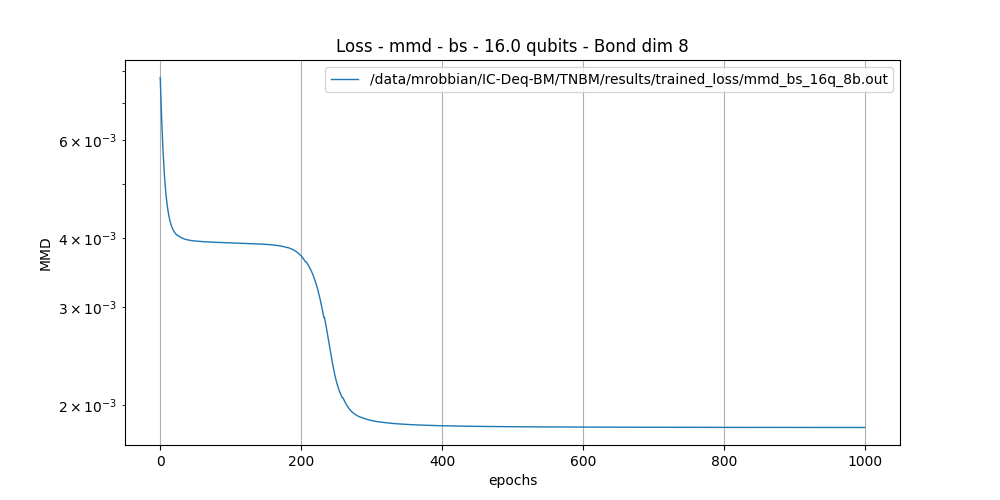
\includegraphics[width=\textwidth]{images/loss_plot/loss_mmd_bs_16.0q_8b_2000i.png}
        \caption{Training progress using MMD loss.}
    \end{subfigure}
    \hfill
    \begin{subfigure}[b]{\textwidth}  
        \centering
        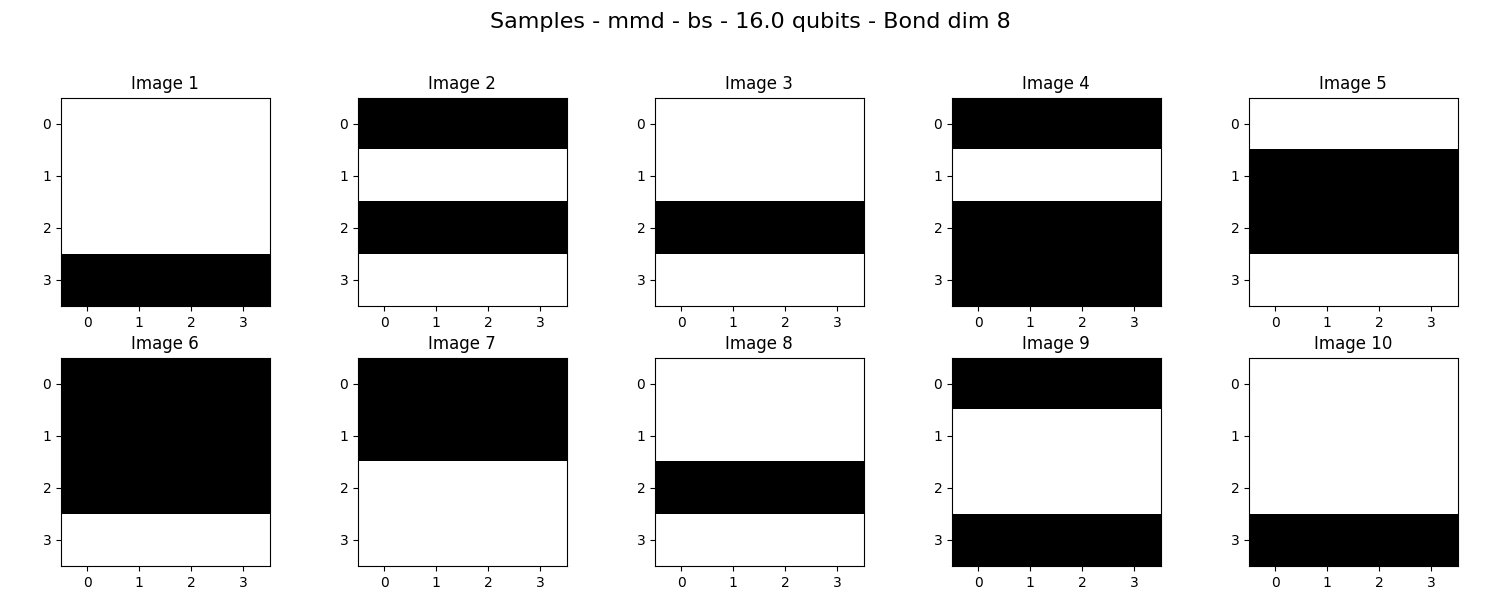
\includegraphics[width=\textwidth]{images/sample_plot/samples_mmd_bs_16.0q_8b_2000i.png}
        \caption{Generated samples using MMD loss.}
    \end{subfigure}
    \caption{Training results and corresponding generated samples for MMD-based training.}
    \label{fig:training_mmd}
\end{figure}

For DKL-based training, we compute the divergence for each bitstring, sum over all samples, and normalize by the total number of samples. Figure~\ref{fig:training_} shows the training evolution and generated samples when optimizing with the DKL loss.

\begin{figure}[h]
    \centering
    \begin{subfigure}[b]{\textwidth}  
        \centering
        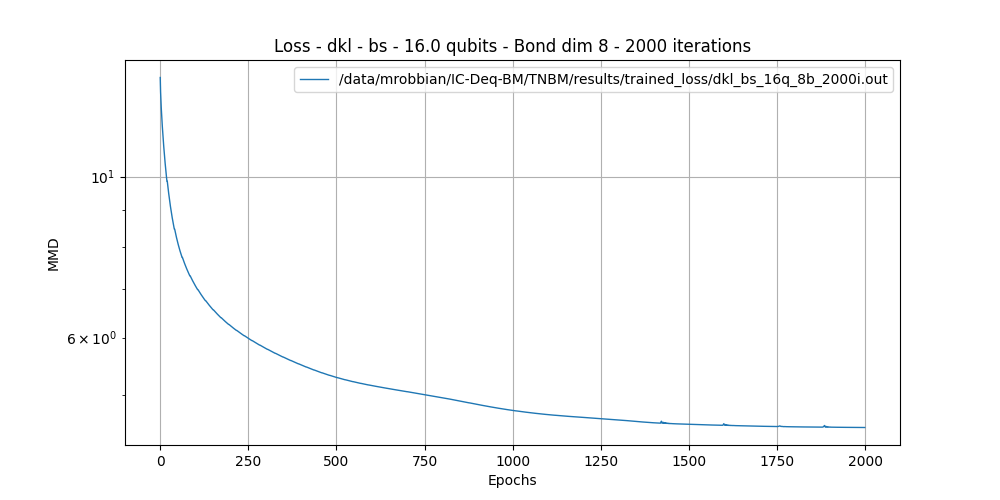
\includegraphics[width=\textwidth]{images/loss_plot/loss_dkl_bs_16.0q_8b_2000i.png}
        \caption{Training progress using DKL loss.}
    \end{subfigure}
    \hfill
    \begin{subfigure}[b]{\textwidth}  
        \centering
        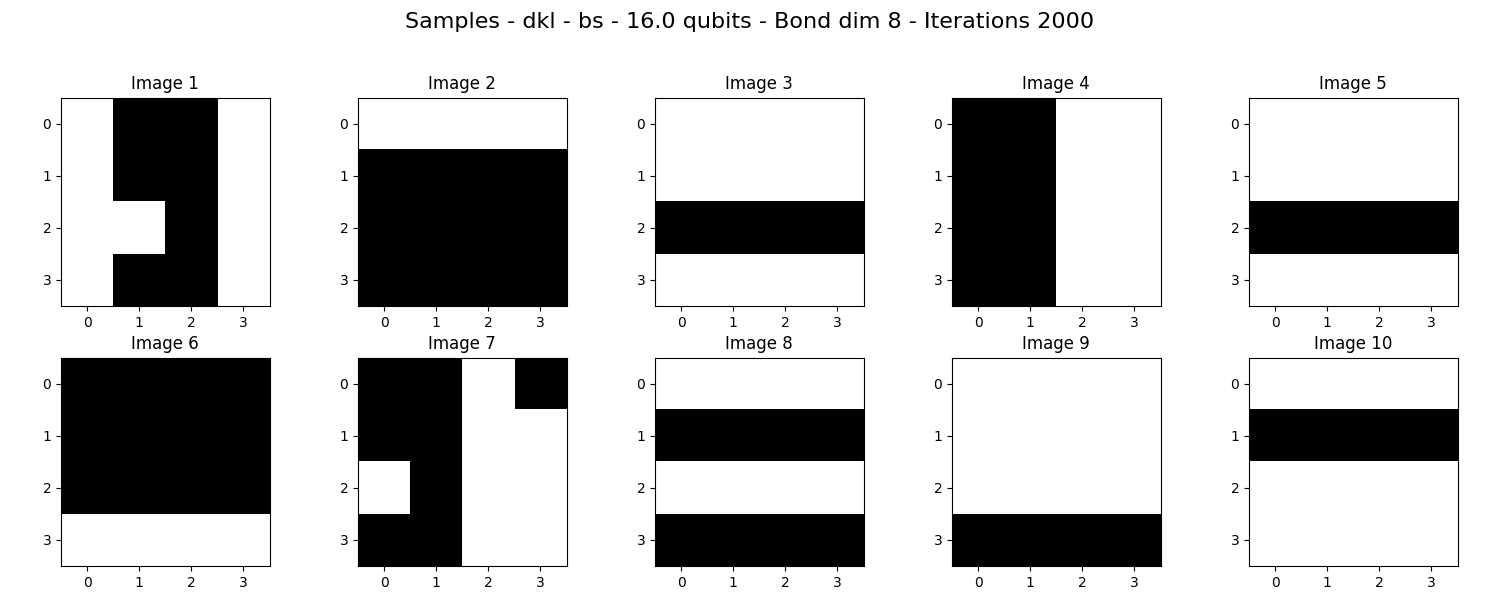
\includegraphics[width=\textwidth]{images/sample_plot/samples_dkl_bs_16.0q_8b_2000i.png}
        \caption{Generated samples using DKL loss.}
    \end{subfigure}
    \caption{Training results and corresponding generated samples for DKL-based training.}
    \label{fig:training_dkl}
\end{figure}
From the training results, we observe that the model trained with the MMD loss exhibits superior performance compared to the one trained with DKL, given the same number of iterations. This improvement is evident both in the loss trajectory, which shows more stable convergence, and in the generated samples, which more accurately reflect the structure of the target distribution. As discussed in the previous chapter, MMD is generally an implicit method. However, in our case, due to the nature of tensor networks, we have formulated it in an explicit manner. 

Previous work \cite{rudolph_trainability_2024} has indicated that it can yield improved performance in certain contexts. Our results are in line with these findings, suggesting that the MMD-based training may offer advantages even when reinterpreted in an explicit framework. In our case, the tensor network representation allows us to recast the method explicitly, which appears to further benefit the model's performance.

\section{Barren Plateau Analysis}

One of the main challenges in optimizing parametrized quantum models is the presence of barren plateaus, where the gradients of the cost function vanish exponentially with system size, making training intractable. To investigate whether our approach suffers from this phenomenon, we analyze the variance of the loss function under random initialization.

For a fixed bond dimension, we compute the variance of the loss function across different random initializations while increasing the number of qubits. This process is repeated for multiple bond dimensions to assess whether the effect depends on the expressivity of the tensor network. The results, shown in Fig.~\ref{fig:barren_plateau}, indicate that the variance decreases exponentially as the system size grows, suggesting the presence of a barren plateau.
\begin{figure}[h]
    \centering
    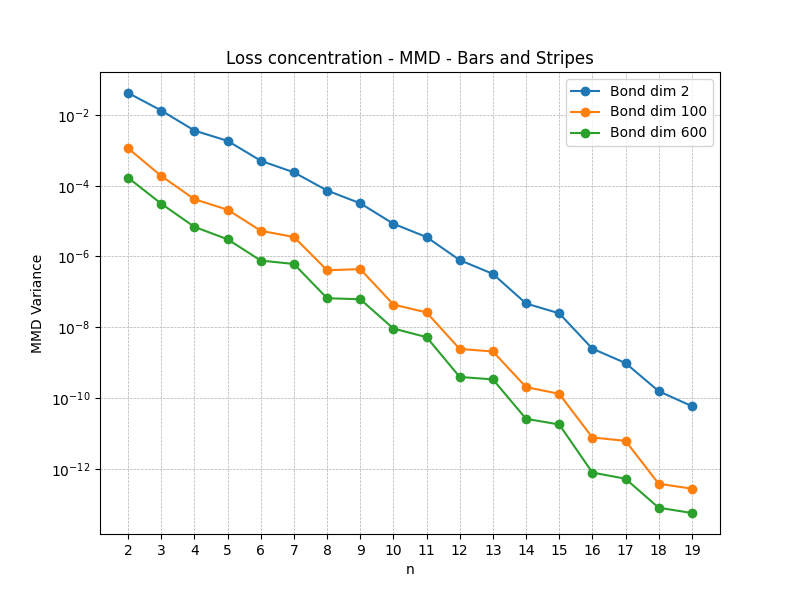
\includegraphics[width=0.7\textwidth]{images/loss_concentration.png}
    \caption{Variance of the loss function at random initialization as a function of the number of qubits, for different bond dimensions. The exponential decay suggests the presence of a barren plateau.}
    \label{fig:barren_plateau}
\end{figure}
Previous work \cite{martin_barren_2023} has shown that while barren plateaus are a known issue for Matrix Product States (MPS), the phenomenon is mitigated when using tensor network architectures such as Tree Tensor Networks (TTN) and Multi-scale Entanglement Renormalization Ansatz (MERA). Our results align with these findings, demonstrating a similar exponential decay in variance for MPS, but with potential for better performance with other tensor network structures.